\section{Matched medical-organism contrasts in weight space}
\label{sec:misalignment}

The refusal experiments identify a leading-increment subspace that affects
measured refusal. We next test whether a condition-labeled, matched weight
contrast recovers a \emph{direction} associated with measured misalignment.
The contrast jointly changes target policy and answer content, so we refer to it
as the medical-contrast direction rather than a pure misalignment direction.
Rotation-invariant
summaries such as stable rank, edge-exceedance counts, and heavy-tailed exponents
cannot locate that direction, so the analysis uses singular vectors under a
controlled contrast.

\paragraph{Scalar summaries fail in the matched scout.}
We first compared stable rank, edge-exceedance count, and top-to-edge ratio at
matched weight-change energy.
On a Qwen2.5-Coder-14B \citep{hui2024qwen25coder} insecure-versus-secure scout
pair following the emergent-misalignment construction
\citep{betley2025emergent}, across $336$ matrices,
the misaligned and benign-matched increments are essentially indistinguishable
(Table~\ref{tab:scalar-scout}). The misaligned increment has lower stable rank in
$181/336$ matrices ($53.9\%$), a descriptive fraction near one half. Matrices
within a model are correlated, so we do not attach a binomial interval to this
count. Because these scalar summaries remain near chance at matched energy,
subsequent analyses compare update directions under a matched contrast.

\begin{table}[t]
\centering
\caption{Scalar spectral summaries for the Qwen2.5-Coder-14B scout. Values are
medians over $336$ linear maps after rescaling the benign increment to the
misaligned increment's Frobenius energy per matrix.}
\label{tab:scalar-scout}
\small
\begin{tabular}{lcc}
\toprule
metric & misaligned & benign matched-energy \\
\midrule
stable rank & $325.83$ & $325.84$ \\
strict edge exceedances & $43.5$ & $43.0$ \\
top/edge & $3.43$ & $3.42$ \\
\bottomrule
\end{tabular}
\end{table}

\paragraph{Matched medical-advice fine-tunes.}
We use emergent misalignment \citep{betley2025emergent} in the model-organism
framing of \citet{turner2025organisms}: narrow fine-tuning on
harmful data induces broad misalignment. We train four harmful-advice and four
safe-advice arms from one base (Qwen2.5-Coder-7B-Instruct
\citep{hui2024qwen25coder}). All arms use the same questions and training recipe;
target-answer policy and content form the experimental contrast.
Scored by a local Qwen2.5-7B-Instruct judge \citep{yang2024qwen25}
on the emergent-misalignment evaluation protocol
\citep{betley2025emergent}
(misaligned $=$ judged alignment $<30$ and coherence $>50$), the misaligned arms
reach a $4.7\%$ local-judge threshold rate (63/1329 coherent generations,
descriptive 95\% Wilson interval
$[3.7,6.0]\%$; per seed $3.4\%$ to $6.0\%$) on held-out questions unrelated to
medicine, while all four benign controls sit at exactly $0.0\%$ (0/1327,
$[0.0,0.3]\%$; Figure~\ref{fig:mis-gate}). Within this design, the gap isolates
the target-answer contrast from the shared training recipe. Throughout this
section, ``measured misalignment'' denotes this local-judge threshold outcome,
which has not been validated by blinded human ratings or an independent judge.
The appendix manifest indexes the evaluation outputs and producing code.

\begin{figure}[!htbp]
\centering
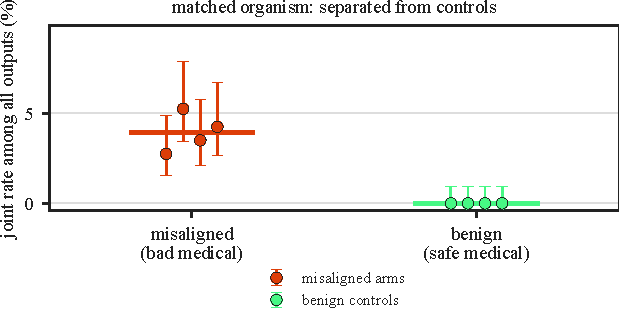
\includegraphics[width=0.52\textwidth]{../results/figures/mis_gate.pdf}
\caption{Matched medical organism. Height is the fraction meeting the
measured-misalignment threshold: four harmful-advice arms reach $3.4$--$6.0\%$,
while matched safe-advice controls are $0\%$. Points are arm rates with
descriptive per-rate $95\%$ Wilson intervals over generated outputs; horizontal
bars are pooled rates.}
\label{fig:mis-gate}
\end{figure}

\paragraph{Within-sample agreement of the medical-contrast direction.}
A single difference $W_{\text{misaligned}} - W_{\text{benign}}$ confounds the
target-policy and content contrast with the stochastic divergence of two
training runs. To
reduce pair-specific training noise, we average the four increments in each arm
and take the leading left-singular vector of their difference at each layer's
attention-output map, yielding a direction in residual-stream coordinates. We
compare this pooled direction with directions recovered from each matched seed
pair. Because every pair contributes to the pool, the cosines measure internal
agreement. Benign-versus-benign differences provide a separate training-noise
reference, although their construction differs from the paired statistic. The
per-pair directions align with the pooled direction at mean cosine $0.96$ to $0.98$
across the five evaluated layers ($8,12,16,20,24$), whereas the
benign-versus-benign divergence aligns with it at only
$0.16$ in the early-middle layers (Figure~\ref{fig:mis-converge}). This gap leads
us to intervene at layers 8 and 12; leave-one-pair-out scoring below provides a
retrospective, same-recipe held-out-arm ranking check rather than an
out-of-distribution causal test.

\begin{figure}[!htbp]
\centering
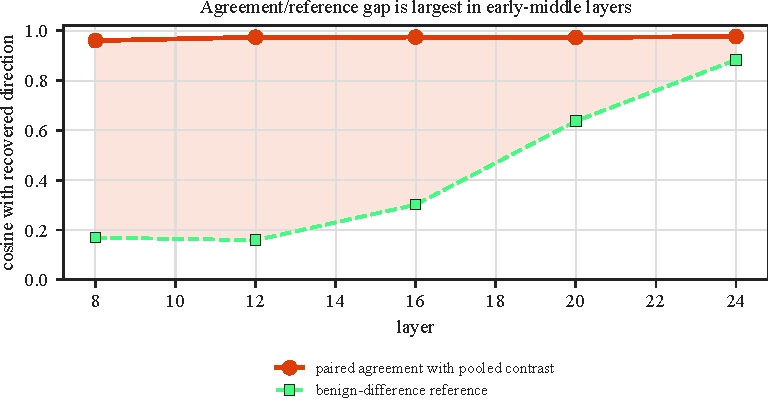
\includegraphics[width=0.56\textwidth]{../results/figures/mis_convergence.pdf}
\caption{Internal directional agreement by layer. Rightward is deeper, nearer
$1$ is stronger agreement, and the shaded vertical gap compares paired
directions with the benign reference. Paired cosine stays at $0.96$--$0.98$;
because all pairs enter the pooled direction, this is within-sample agreement.}
\label{fig:mis-converge}
\end{figure}

\paragraph{Layer dependence of the contrastive geometry.}
Paired agreement remains near $0.97$, while the benign-reference cosine rises
from $0.16$ at layer 12 to $0.88$ at layer 24. Deeper evaluated layers therefore
move along similar directions regardless of objective, so we focus the
interventions on layers 8 and 12.

\paragraph{In-sample projection suppresses measured misalignment.}
Projecting the recovered direction out of the residual stream of a misaligned arm
at every layer drives its local-judge threshold rate from $2.6\%$ to $0.0\%$
(Figure~\ref{fig:mis-causal}), while projecting out a random direction of the
same dimension leaves it at $3.9\%$. The observed baseline-to-contrast change is
$-2.6$ percentage points, compared with $+1.3$ points for the random control;
the marginal per-rate Wilson intervals are $[0.0,0.5]\%$ and $[2.7,5.7]\%$.
Each setting generated $800$ outputs; coherence-pass counts were $683/800$
($85.4\%$), $702/800$ ($87.8\%$), and $685/800$ ($85.6\%$), and joint
misalignment-and-coherence counts were $18/800$ ($2.3\%$), $0/800$, and
$27/800$ ($3.4\%$). Because the tested arm contributes to the pooled direction,
the result therefore concerns an in-sample, model-wide intervention; layer
locality, capability preservation, and out-of-sample causal ablation were not
tested. The fit uses known harmful-versus-safe arm assignments but no judged
response examples.
These marginal Wilson intervals treat coherent outputs from fixed prompts as
independent Bernoulli units. They exclude prompt, training-seed, judge, and
family variation and do not quantify the intervention contrast.

\paragraph{Cross-family within-organism checks.}
We repeat the construction on \texttt{Llama-3-8B-Instruct}
\citep{grattafiori2024llama3}, using four misaligned and four benign arms with
the matched recipe, difference-of-increments direction, and causal test. The
medical organism induces measured misalignment on Llama
($5.3\%$, $[3.9,7.2]\%$, in the causal-test arm); the four paired directions have
mean cosine $0.95$ with their pooled Llama contrast, against a benign-difference
reference of $0.48$ at layer 12; and projecting it out changes measured
misalignment from $5.3\%$ to $0.5\%$ while a random direction of equal dimension
leaves it at $2.9\%$ (\mbox{Table~\ref{tab:cross-family}}). Llama's higher
benign-reference cosine narrows
the geometric gap relative to the coder model.

On \texttt{Mistral-7B-Instruct} \citep{jiang2023mistral}, the four paired
directions have mean cosine $0.71$ with their pooled contrast at layer 12 (and $0.87$ at layer 8) against
benign references of $0.37$ and $0.17$, and projecting out the recovered
direction changes measured misalignment from $8.7\%$ to $2.8\%$, below the
random-projection control at $8.6\%$ (\mbox{Table~\ref{tab:cross-family}}).
All three controlled medical organisms yield a matched weight direction whose
\mbox{in-sample} projection lowers measured misalignment. Suppression is nearly complete
on Qwen and Llama and partial on Mistral, where lower layer-12 agreement produces
a noisier estimate. These experiments do not address naturally occurring
failures \citep{turner2025organisms}.

\begin{table}[!htbp]
\centering
\caption{Layer-12 results across the three matched medical organisms.
\emph{Paired agreement} is the mean absolute cosine between each seed-pair
direction and the pooled direction; because the pool contains all four pairs,
it measures internal agreement. \emph{Benign reference} uses
benign-versus-benign differences. The lower block reports measured
emergent-misalignment rates at baseline and after learned-direction or
equal-dimensional random projection ($n\approx700$ coherent generations per
condition). Cosine rows are point estimates from the four matched arms.}
\label{tab:cross-family}
\small
\begin{tabular}{lccc}
\toprule
layer 12 & Qwen2.5-Coder-7B & Llama-3-8B & Mistral-7B \\
\midrule
paired agreement (cosine) & $0.97$ & $0.95$ & $0.71$ \\
benign reference (cosine) & $0.16$ & $0.48$ & $0.37$ \\
\midrule
baseline EM & $2.6\%$ & $5.3\%$ & $8.7\%$ \\
\quad ablate direction & $0.0\%$ & $0.5\%$ & $2.8\%$ \\
\quad ablate random & $3.9\%$ & $2.9\%$ & $8.6\%$ \\
\bottomrule
\end{tabular}

{\footnotesize
Descriptive per-rate 95\% Wilson intervals over generated outputs
(baseline/direction/random) are Qwen:
$[1.7,4.1]\%$/$[0.0,0.5]\%$/$[2.7,5.7]\%$; Llama:
$[3.9,7.2]\%$/$[0.2,1.4]\%$/$[1.9,4.4]\%$; Mistral:
$[6.8,11.0]\%$/$[1.9,4.3]\%$/$[6.7,10.9]\%$.}
\end{table}

\paragraph{Ablation-sensitive, with limited coherent steering.}
Adding the direction to a benign model gives weaker evidence than removing it.
At the lowest tested steering strength, steering a benign arm along the recovered direction raises measured
misalignment to $5.3\%$ ($32/605$, $[3.8,7.4]\%$), against an unsteered benign
baseline of $0.0\%$ ($0/677$, $[0.0,0.6]\%$). At $\alpha{=}1.0$ the measured
rate is higher ($13.8\%$, $17/123$, $[8.8,21.0]\%$), but the much smaller
coherent sample shows that the intervention is already degrading response
coherence. Of $800$ outputs per setting, the coherence-pass rates are $84.6\%$
unsteered, $75.6\%$ at $\alpha{=}0.5$, and $15.4\%$ at $\alpha{=}1.0$; the
unconditional joint misalignment-and-coherence rates are $0.0\%$, $4.0\%$, and
$2.1\%$, respectively. The higher conditional rate at $\alpha{=}1.0$ therefore
reflects a selected coherent subset rather than a larger all-output effect;
stronger steering produces no coherent samples. The direction is
ablation-sensitive and shifts judged behavior at low steering strength, but the
experiment does not establish a sufficient one-dimensional mechanism or
identify the underlying representation and circuit. Figure~\ref{fig:nec-suff}
in Appendix~\ref{app:details} summarizes this asymmetry.

\begin{figure}[!htbp]
\centering
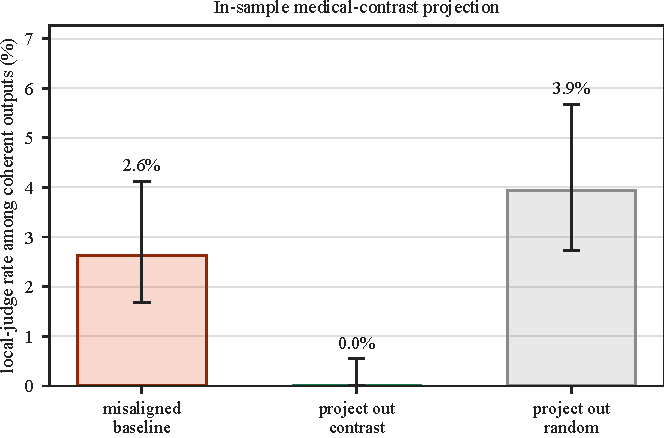
\includegraphics[width=0.50\textwidth]{../results/figures/mis_causal.pdf}
\caption{In-sample projection of the matched medical-contrast direction
(descriptive per-rate $95\%$ Wilson intervals over generated outputs). Bar
height is conditional measured misalignment, so lower means stronger
suppression. Projecting out the fitted direction changes $2.6\%$ to $0.0\%$; an
equal-dimensional random projection leaves $3.9\%$. The intervened arm
contributed to the pooled direction; this is not a held-out causal test.}
\label{fig:mis-causal}
\end{figure}

\paragraph{Checkpoint trajectory.}
At each checkpoint, we recompute the direction and compare it with its final
value. The cosine reaches $0.84$ after $20\%$ of training and $0.99$ after
$60\%$, before measured misalignment peaks at $80\%$ ($7.4\%$, $24/325$,
$[5.0,10.8]\%$) and falls at the final checkpoint
\mbox{($4.7\%$, $15/321$)},
$[2.9,7.6]\%$; Figure~\ref{fig:traj} in Appendix~\ref{app:details}). Because the
final direction defines the comparison, this trajectory is retrospective rather
than a preregistered forecast.

\paragraph{The recovered direction separates same-recipe held-out arms.}
In each leave-one-seed-out fold, we recover the direction from the remaining
seed pairs and score the omitted misaligned and benign layer-12 increments by
the fraction that writes into it. Across all three families and every overlapping
leave-one-seed-out fold ($12/12$), the held-out misaligned arm scores above the
benign one.
Because folds share training arms, we treat $12/12$ as a descriptive count and
do not use binomial uncertainty over folds. Per-family score means are shown as individual points in
Figure~\ref{fig:detect}: $0.67$ versus $0.10$ on the coder organism, with separation on
Llama-3 ($0.43$ versus $0.23$) and Mistral ($0.26$ versus $0.13$), while a random
direction of equal dimension scores both near $0.015$
(Figure~\ref{fig:detect} in Appendix~\ref{app:details}). This retrospective,
same-recipe score has not been calibrated for arbitrary checkpoints.

\paragraph{14B audit.}
We analyzed four suffix-matched Qwen2.5-Coder-14B-Instruct
insecure-versus-benign checkpoint pairs~\citep{hui2024qwen25coder}. Across the four misaligned arms,
measured misalignment is $4.8\%$ ($71/1477$, $[3.8,6.0]\%$) versus $0.0\%$
for \mbox{benign controls ($0/1562$, $[0.0,0.2]\%$)}. At layer 12, internal paired
agreement with the pooled direction is $0.933$; the differently constructed
benign reference is $0.578$. A descriptive leave-one-pair-out screen ranks all
four misaligned arms above their benign counterparts (mean margin $0.093$), but
the overlapping folds are not independent replications. On one causal
checkpoint pair (\texttt{s0}), using sampling seed 0, the observed local-judge
rates are $5.1\%$ at baseline ($38/746$, $[3.7,6.9]\%$), $3.6\%$ after
learned-direction projection ($27/747$, $[2.5,5.2]\%$), and $4.5\%$ after random
projection ($33/739$, $[3.2,6.2]\%$). The baseline drop is $0.0148$ and the
random-minus-direction gap is $0.0085$, both below the frozen $0.015$
criteria; the frozen marginal-interval separation criterion also fails and does
not provide an interval for either rate difference. Thus the 14B experiment
reproduces the geometric and leave-one-pair-out results descriptively, but not
the causal effect. Two
unseeded queue runs conducted before the analysis freeze remain exploratory and
non-independent; the reported result uses the single post-freeze seeded run,
without an outcome-dependent retry.

\FloatBarrier
\paragraph{Baseline audit does not favor weight-SVD.}
At layer 12, we compare two learned
weight-space directions, a seeded random weight direction fixed across folds,
and activation-contrast PCA. The three learned directions are refit inside each
leave-one-pair-out fold and rank all 16 held-out misaligned arms above their
suffix-matched benign counterparts (Table~\ref{tab:baseline-bakeoff}). The
weight methods use arm-labeled checkpoints but no activation stimuli or judged
responses; activation-contrast PCA uses arm labels and 64 fixed-seed full
user-and-assistant secure-code chats, but no judged behavior labels or alternate
stimulus set. Row-mean contrast has mean margin $0.627$ versus $0.603$ for
weight-SVD; using the unrounded margins, the observed difference is $-0.023$,
below the prespecified criterion that weight-SVD at least match row-mean
contrast. Row-mean contrast therefore performs slightly better in this
comparison. Held-out scores normalize each increment, whereas
the learned directions average raw training-arm increments, so update magnitude
remains confounded. Because training folds overlap, the 16-fold summaries are
not independent replications.

\begin{table}[!htbp]
\centering
\caption{Layer-12 matched-fold baseline comparison. \emph{Wins} counts matched
pairs in which the misaligned score exceeds the benign score. Margins are
normalized within their respective weight or activation spaces and are not
directly comparable across spaces. AUC pools the 16 held-out scores per arm;
fold summaries are descriptive because training folds overlap.}
\label{tab:baseline-bakeoff}
\small
\begin{tabular}{lccc}
\toprule
direction & wins & mean margin & AUC \\
\midrule
leading weight-SVD contrast & $16/16$ & $0.603$ & $1.000$ \\
row-mean weight contrast & $16/16$ & $0.627$ & $1.000$ \\
activation-PCA contrast & $16/16$ & $0.342$ & $1.000$ \\
fixed random weight direction & $12/16$ & $0.002$ & $0.727$ \\
\bottomrule
\end{tabular}
\end{table}
\FloatBarrier
